\documentclass[border=12pt,tikz]{standalone}
\usepackage[T1]{fontenc}
\usepackage{helvet}
\renewcommand{\familydefault}{\sfdefault}
\usepackage{sfmath}
\usepackage{tikz}
\usepackage{xcolor}

\usetikzlibrary{arrows.meta, calc, positioning, fit, backgrounds}

% ── palette ─────────────────────────────────────────────────────
\definecolor{fgdark}{HTML}{1F2328}
\definecolor{fgmuted}{HTML}{656D76}
\definecolor{edgecol}{HTML}{8C959F}

% category: authored (user's own)
\definecolor{authfill}{HTML}{D97706}
\definecolor{authline}{HTML}{B45309}
% category: contributed
\definecolor{contfill}{HTML}{0E7490}
\definecolor{contline}{HTML}{155E75}
% category: used (external)
\definecolor{usedfill}{HTML}{EAECEF}
\definecolor{usedline}{HTML}{C2C8CF}

% group boxes
\definecolor{grpline}{HTML}{B0B7BF}

\tikzset{
  pkg/.style={
    rounded corners=4pt, draw, line width=1.1pt,
    minimum height=9mm, minimum width=20mm, inner xsep=7pt,
    font=\small\ttfamily,
  },
  authored/.style={pkg, fill=authfill, draw=authline, text=white},
  contributed/.style={pkg, fill=contfill, draw=contline, text=white},
  used/.style={pkg, fill=usedfill, draw=usedline, text=fgdark},
  dep/.style={-{Stealth[length=6pt,width=4.5pt]}, line width=1.3pt, edgecol},
  trunk/.style={line width=1.3pt, edgecol},
  grp/.style={rounded corners=6pt, draw=grpline, line width=1pt, dash pattern=on 3pt off 2pt},
  grplab/.style={font=\footnotesize\sffamily\itshape, text=fgmuted},
}

\begin{document}
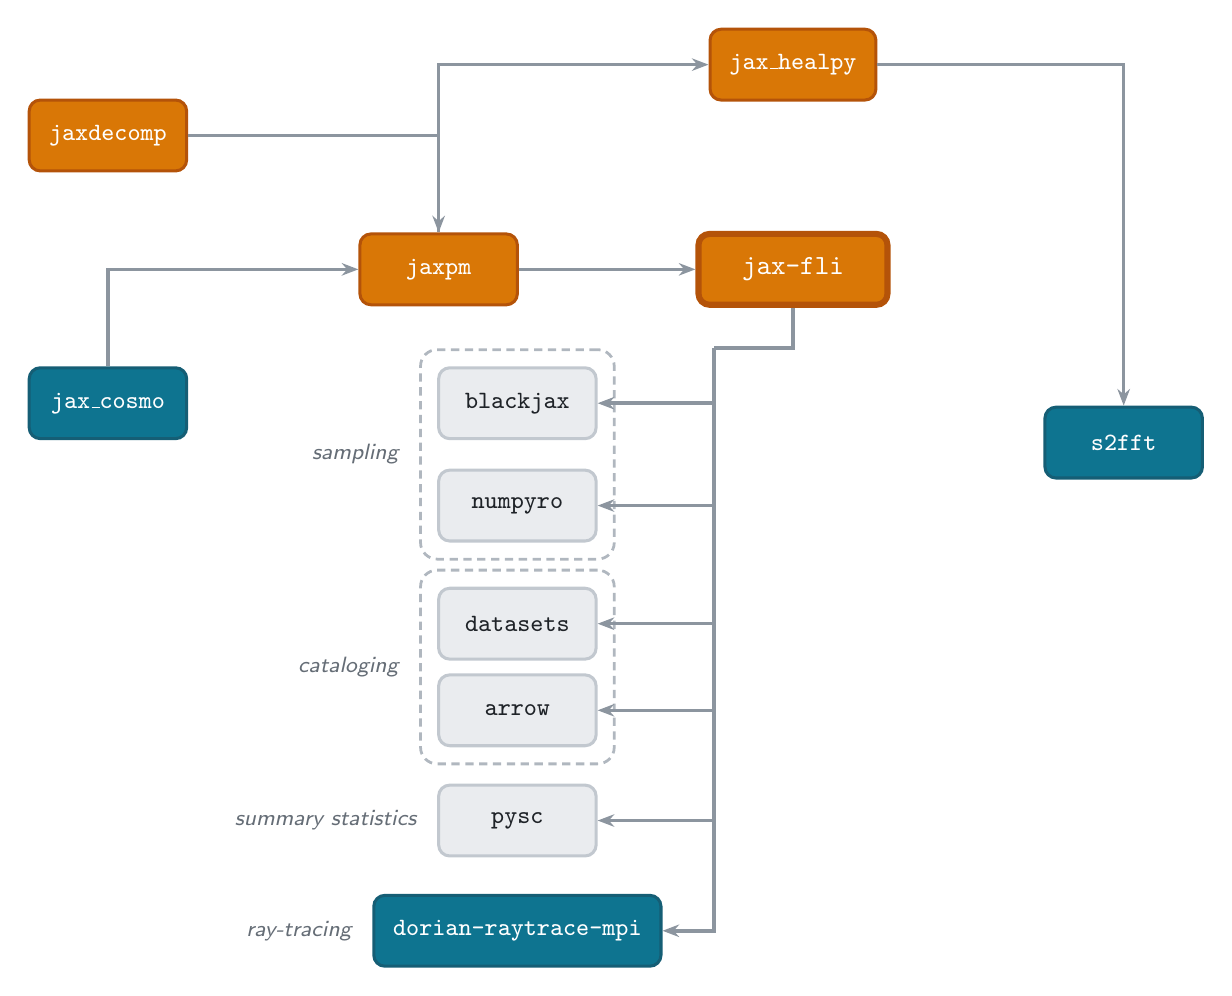
\begin{tikzpicture}[node distance=6mm]

% ── foundations (left) ─────────────────────────────────────────
\node[authored] (jaxdecomp) at (0, 1.7) {jaxdecomp};
\node[contributed] (jaxcosmo) at (0, -1.7) {jax\_cosmo};

% ── jaxPM ───────────────────────────────────────────────────────
\node[authored] (jaxpm) at (4.2, 0) {jaxpm};

% ── spherical-harmonics branch (up) ─────────────────────────────
\node[authored]    (jaxhp)  at (8.7, 2.6) {jax\_healpy};
\node[contributed] (s2fft)  at (12.9, -2.2) {s2fft};

% ── jax-fli (hub) ───────────────────────────────────────────────
\node[authored, minimum width=24mm, line width=2.2pt, font=\normalsize\ttfamily\bfseries]
  (jaxfli) at (8.7, 0) {jax-fli};

% ── outputs (stacked DOWN, left-of-hub) ─────────────────────────
\node[used] (blackjax) at (5.2, -1.7) {blackjax};
\node[used] (numpyro)  at (5.2, -3.0) {numpyro};
\node[used] (datasets) at (5.2, -4.5) {datasets};
\node[used] (arrow)    at (5.2, -5.6) {arrow};
\node[used]        (pysc)   at (5.2, -7.0) {pysc};
\node[contributed] (dorian) at (5.2, -8.4) {dorian-raytrace-mpi};

% ── dependency edges (orthogonal: 0/90 deg only) ────────────────
\draw[dep] (jaxdecomp.east) -| (jaxpm.north);
\draw[dep] (jaxcosmo.north) |- (jaxpm.west);
\draw[dep] (jaxpm.east) -- (jaxfli.west);
\draw[dep] (jaxpm.north) |- (jaxhp.west);
\draw[dep] (jaxhp.east) -| (s2fft.north);

% distribution bus for jaxfli outputs (drops down, right-side rail)
\coordinate (obus) at (7.7,-1.0);
\draw[trunk] (jaxfli.south) |- (obus);
\draw[dep] (obus) |- (blackjax.east);
\draw[dep] (obus) |- (numpyro.east);
\draw[dep] (obus) |- (datasets.east);
\draw[dep] (obus) |- (arrow.east);
\draw[dep] (obus) |- (pysc.east);
\draw[dep] (obus) |- (dorian.east);

% ── purpose group boxes ─────────────────────────────────────────
\begin{scope}[on background layer]
  \node[grp, fit=(blackjax)(numpyro), inner sep=6pt] (sampbox) {};
  \node[grp, fit=(datasets)(arrow),   inner sep=6pt] (catbox)  {};
\end{scope}
\node[grplab, anchor=east] at ([xshift=-4pt]sampbox.west) {sampling};
\node[grplab, anchor=east] at ([xshift=-4pt]catbox.west)  {cataloging};
\node[grplab, anchor=east] at ([xshift=-4pt]pysc.west)    {summary statistics};
\node[grplab, anchor=east] at ([xshift=-4pt]dorian.west)  {ray-tracing};

\end{tikzpicture}
\end{document}
